% !TEX program = xelatex
\documentclass[hyperref,a4paper,UTF8]{ctexart}

\usepackage[left=2.50cm, right=2.50cm, top=2.50cm, bottom=2.50cm]{geometry}

\usepackage[unicode=true,colorlinks,urlcolor=blue,linkcolor=blue,bookmarksnumbered=true]{hyperref}
\usepackage{latexsym,amssymb,amsmath,amsbsy,amsopn,amstext,amsthm,amsxtra,color,bm,calc,ifpdf}
\usepackage{graphicx}
\usepackage{enumerate}
\usepackage{fancyhdr}
\usepackage{listings}
\usepackage{multirow}
\usepackage{makeidx}
\usepackage{xcolor}
\usepackage{fontspec}
\usepackage{subfigure}
\usepackage{hyperref}
\usepackage{pythonhighlight}
\usepackage{cite}
\usepackage[justification=centering]{caption}
\usepackage{pifont}
\usepackage{enumitem}
\usepackage{longtable}
\usepackage{makecell}


\lstset{
    xleftmargin=8em, xrightmargin=6em, aboveskip=1em,
    framexleftmargin=2em,
    basicstyle=\footnotesize,
    numbers=left,
    numberstyle=\tiny\color{gray},
    backgroundcolor=\color{white},
    showspaces=false,
    showstringspaces=false,
    showtabs=false,
    frame=single,
    rulecolor=\color{black},
    tabsize=4,
    captionpos=b,
    breaklines=true,
    breakatwhitespace=false,
    title=\lstname,
    keywordstyle=\color{blue},
    commentstyle=\color{dkgreen},
    stringstyle=\color{mauve},
    escapeinside={\%*}{*},
    morekeywords={*,...}
}

\pagestyle{fancy}
\fancyhead[L]{}
\fancyhead[C]{\fangsong 汽车公司管理系统设计 \quad 数据库系统原理期末项目报告}
\fancyhead[R]{}


\title{\textbf{{汽车公司管理系统} \\ \large{数据库系统原理期末项目报告}}}
\author{
\kaishu\normalsize
姓名\ \underline{黄灿彬} \qquad
学号\ \underline{20337039} \qquad
院系\ \underline{计算机学院}
}
\date{} % 留空,不显示日期


\begin{document}

\begin{figure}
    \centering
    
\includegraphics[width=0.65\textwidth]{figures/sysu.png}
\end{figure}

\maketitle

\

\tableofcontents

\thispagestyle{empty} % 当前页不显示页码
\newpage

\section{需求分析和系统设计}

\subsection{需求分析}

本项目需要利用数据库实现一个汽车公司管理系统,在数据库中需要记录品牌、车型、车辆、顾客、经销商、销售记录等信息。该系统需要提供数据库管理、车辆库存查询、销量记录和统计分析等功能;并且,该系统需要有不同的应用界面以供不同类型的用户访问数据库:

\begin{itemize}[itemsep=2pt,topsep=0pt,parsep=0pt]
    \item \textbf{数据库管理员}需要使用 SQL 管理数据库;
    \item \textbf{经销商}需要查询自己或附近经销商的库存从而找到复合顾客需求的汽车;
    \item \textbf{顾客}需要通过一个网页界面来查询经销商和汽车;
    \item \textbf{公司市场部}需要使用数据库的 OLAP 功能来生成销量报告或对特定数据进行分析,他们还希望能够通过经销商的查询请求来决定未来的生产计划。
\end{itemize}

\subsection{系统设计}

根据以上需求分析,本项目使用 MySQL 作为数据库管理系统,并开发一个网站作为应用界面来支持不同类型用户的不同需求。系统总体结构如下:

\begin{figure}[h]
    \centering
    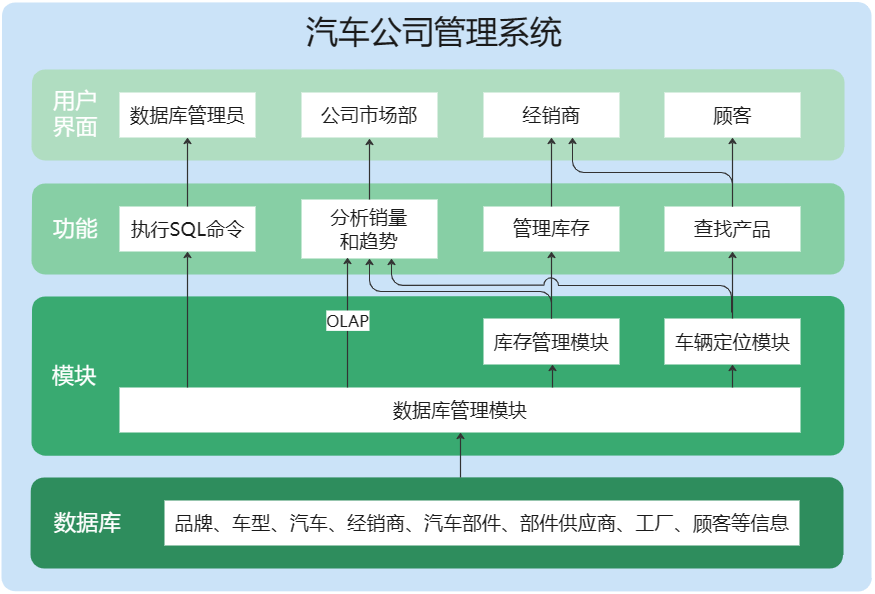
\includegraphics[width=\textwidth]{figures/系统结构图.png}
    \caption{汽车公司管理系统结构图}
    \label{fig:汽车公司管理系统结构图}
\end{figure}

如图\ref{fig:汽车公司管理系统结构图}所示,本系统包含 4 个部分。其中,用于存储信息的数据库由 MySQL 提供支持,数据库的设计将在第\ref{sec:数据库设计}节详细阐述。而用户界面、功能和模块需编写 python 程序实现,将在第\ref{sec:应用程序设计}节详细阐述。最后,第\ref{sec:功能展示和测试}节将展示系统的使用方法并通过几个测试来证明本系统的正确性和实用性。

\section{数据库设计\label{sec:数据库设计}}

\subsection{E-R 模型\label{sec:E-R模型}}

\subsubsection{E-R 图}

\begin{figure}[h]
    \centering
    \includegraphics[width=\textwidth]{figures/ER图.png}
    \caption{汽车公司数据库 E-R 图}
    \label{fig:ER图}
\end{figure}

图\ref{fig:ER图}为汽车公司数据库的 E-R 图,图中符号含义如下:

\begin{itemize}[itemsep=2pt,topsep=0pt,parsep=0pt]
    \item 带有一半阴影的矩形表示实体集,阴影部分为实体集名字,空白部分为属性;
    \item 菱形表示联系集;
    \item 双菱形表示连接到弱实体集的标志性联系集;
    \item 不带阴影的矩形表示联系集属性;
    \item 线段将实体集连接到联系集,一个二元联系集的两个线段都带箭头表示一对一关系,只有一个带有箭头表示一对多关系,两个都没有箭头表示多对多关系;
    \item 虚线将联系集属性连接到联系集;
    \item 双线表示实体集中的实体在联系集中全部参与;
    \item 无法用双线和箭头表示的映射基数在线段上用\textit{l..h}表示,其中,\textit{l}表示最小映射基数,\textit{r}表示最大映射基数。
\end{itemize}

\subsubsection{实体集}

E-R 图中的实体集如下:

\begin{itemize}[itemsep=2pt,topsep=0pt,parsep=0pt]
    \item \textit{Brand}:品牌,包含属性\textit{(\underline{BID}, name)};
    \item \textit{Model}:车型,包含属性\textit{(\underline{MID}, name, body\_style)};
    \item \textit{Option}:选项组合,一个车型可能提供颜色、引擎、变速器不同的汽车,这是一个依赖于\textit{Model}的弱实体集,包含属性\textit{(\underline{color}, \underline{engine}, \underline{transmission})};
    \item \textit{Part}:汽车部件,包含属性\textit{(\underline{model}, name, info)},一种部件可以由公司自己的工厂生产,也可以由供应商提供,注意这里的属性\textit{model}是指部件的型号而不是车型;
    \item \textit{Supplier}:供应商,向汽车公司供应汽车部件,包含属性\textit{(\underline{supplier\_name}, address(country, city, street))};
    \item \textit{Plant}:汽车公司自己所有的工厂,包含属性\textit{(\underline{plant\_name}, work\_type, address(country, city, street))},其中,\textit{work\_type}表示该工厂是生产汽车部件还是组装汽车;
    \item \textit{Vehicle}:汽车,包含属性\textit{(\underline{VIN}, price)};
    \item \textit{Dealer}:经销商,包含属性\textit{(\underline{DID}, name, area(country, city))};
    \item \textit{Customer}:顾客,包含属性\textit{(\underline{CID}, name, address(country, city, street), \{phone\}, gender, annual\_income)},由于一位顾客可能有不止一个电话号码,所以\textit{phone}是多值属性。
\end{itemize}

\subsubsection{联系集\label{sec:relationship-set}}

E-R 图中的联系集以及对应的映射基数和参与约束解释如下:

\begin{itemize}[itemsep=2pt,topsep=0pt,parsep=0pt]
    \item \textit{model\_brand}:关联\textit{Model}和\textit{Brand},表示一个车型所属的品牌,一个品牌可能提供多种车型,但每个车型必定属于一个品牌,所以,\textit{model\_brand}和\textit{Brand} 之间是箭头,而\textit{model\_brand}和\textit{Model} 之间是双线,下面同理;
    \item \textit{model\_op}:关联\textit{Model}和\textit{Option},表示一个车型提供的选项组合,一个车型可能提供多种选项,但是一个选项必定由一个车型提供;
    \item \textit{requires}:关联\textit{Model}和\textit{Part},表示一个车型需要的部件,一个车型需要多个部件,一个部件也可能提供给多个车型;
    \item \textit{supplies}:关联\textit{Supplier}和\textit{Part},表示一个供应商提供的部件,一个供应商可能提供多种部件,一种部件也可能由多个供应商提供;
    \item \textit{manufactures}:关联\textit{Plant}和\textit{Part},表示一个工厂生产的部件,一个工厂可能生产多种部件或不生产部件,一种部件可能由多个工厂生产;
    \item \textit{made\_of}:关联\textit{Vehicle}和\textit{Part},表示一辆汽车由哪些部件组装成,描述属性\textit{manufacturer}和\textit{manu\_date(year, month, day)}分别表示该部件的制造商和制造日期,其中制造日期是一个复合属性,每辆汽车都是由部件构成的,但是一个部件未必已经装在一辆汽车上;
    \item \textit{assembles}:关联\textit{Plant}和\textit{Vehicle},表示汽车是由哪个工厂组装的,描述属性\textit{assem\_data(year, month, day)}表示组装日期,每辆汽车都是在工厂中组装的,但是有的工厂可能不组装汽车;
    \item \textit{vehicle\_op}:关联\textit{Vehicle}和\textit{Option},表示汽车属于哪种车型和选项组合,每辆汽车都属于一种选项组合,而一种选项组合可能有多辆汽车;
    \item \textit{inventory}:关联\textit{Dealer}和\textit{Vehicle},表示经销商的进货记录,描述属性\textit{date}和\textit{is\_sold}和分别表示该汽车的进货日期和是否已经卖出;
    \item \textit{sales}:关联\textit{Brand}、\textit{Model}和\textit{Dealer},表示某个品牌和车型的某种颜色的车在某个经销商处某一天的销量;
    \item \textit{sell}:关联\textit{Dealer}、\textit{Vehicle}和\textit{Customer},表示某个经销商在某一天把某辆汽车卖给了某个客户。
\end{itemize}

\subsection{关系模式}

\subsubsection{将 E-R 图转换为关系模式}

将\ref{sec:E-R模型}节中的 E-R 模型直接转换为关系模式,注意对于复合属性、多值属性和弱实体集的处理:

\begin{center}
    \begin{tabular}{l}
        Brand(\underline{BID}, name)\\
        Model(\underline{MID}, name, body\_style)\\
        Option(\underline{MID}, \underline{color}, \underline{engine}, \underline{transmission})\\
        Part(\underline{model}, name, info)\\
        Supplier(\underline{supplier\_name}, country, city, street)\\
        Plant(\underline{plant\_name}, work\_type, country, city, street)\\
        Vehicle(\underline{VIN}, price)\\
        Dealer(\underline{DID}, name, country, city)\\
        Customer(\underline{CID}, name, country, city, street, gender, annual\_income)\\
        customer\_phone(\underline{CID}, \underline{phone})\\
        model\_brand(\underline{MID}, BID)\\
        model\_op(\underline{MID}, \underline{color}, \underline{engine}, \underline{transmission})\\
        requires(\underline{MID}, \underline{part\_model})\\
        supplies(\underline{supplier\_name}, \underline{part\_model})\\
        manufactures(\underline{plant\_name}, \underline{part\_model})\\
        made\_of(\underline{VIN}, \underline{part\_model}, manufacturer, year, monty, day)\\
        assembles(\underline{VIN}, plant\_name)\\
        vehicle\_op(\underline{VIN}, \underline{MID}, \underline{color}, \underline{engine}, \underline{transmission})\\
        inventory(\underline{VIN}, DID, year, monty, day, is\_sold)\\
        sales(\underline{BID}, \underline{MID}, \underline{color} \underline{DID}, \underline{year}, \underline{monty}, \underline{day}, quantity)\\
        sells(\underline{VIN}, DID, CID, year, monty, day)
    \end{tabular}
\end{center}

\subsubsection{对关系模式进行优化\label{sec:对关系模式进行优化}}

注意到由 E-R 图转换的关系模式中存在许多冗余,例如,关系模式 model\_op 的属性不仅和 Option 完全相同,而且每一组属性值都会在 Option 中出现。另外,基于\ref{sec:relationship-set}小节对联系集映射基数和参与约束的分析,可以将 model\_brand 合并到 Model,将 assembles 和 vehicle\_op 合并到 Vehicle。优化后的关系模式如下:

\begin{center}
    \begin{tabular}{l}
        Brand(\underline{BID}, name)\\
        Model(\underline{MID}, name, body\_style, BID)\\
        Option(\underline{MID}, \underline{color}, \underline{engine}, \underline{transmission})\\
        Part(\underline{model}, name, info)\\
        Supplier(\underline{supplier\_name}, country, city, street)\\
        Plant(\underline{plant\_name}, work\_type, country, city, street)\\
        \makecell[l]{Vehicle(\underline{VIN}, price, plant\_name, assembly\_year, assembly\_month, assembly\_day, \\ \qquad \quad \  MID, color, engine, transmission)}\\
        Dealer(\underline{DID}, name, country, city)\\
        Customer(\underline{CID}, name, country, city, street, gender, annual\_income)\\
        customer\_phone(\underline{CID}, \underline{phone})\\
        requires(\underline{MID}, \underline{part\_model})\\
        supplies(\underline{supplier\_name}, \underline{part\_model})\\
        manufactures(\underline{plant\_name}, \underline{part\_model})\\
        made\_of(\underline{VIN}, \underline{part\_model}, manufacturer, year, monty, day)\\
        inventory(\underline{VIN}, DID, year, month, day, is\_sold)\\
        sales(\underline{BID}, \underline{MID}, \underline{color}, \underline{DID}, \underline{year}, \underline{monty}, \underline{day}, quantity)\\
        sells(\underline{VIN}, DID, CID, year, monty, day)
    \end{tabular}
\end{center}

\subsection{SQL}

在本项目中,使用 MySQL 作为数据库管理系统。首先,我们根据\ref{sec:对关系模式进行优化}小节中的关系模式,编写如下 SQL DDL 脚本以创建数据库:

\begin{lstlisting}[language=SQL]
CREATE DATABASE AutomobileCompany;
USE AutomobileCompany;
CREATE TABLE Brand (
    BID VARCHAR(20) NOT NULL,
    name VARCHAR(20) NOT NULL,
    PRIMARY KEY (BID)
);
CREATE TABLE Model (
    MID VARCHAR(20) NOT NULL,
    name VARCHAR(20) NOT NULL,
    body_style VARCHAR(20) NOT NULL,
    BID VARCHAR(20) NOT NULL,
    PRIMARY KEY (MID),
    FOREIGN KEY (BID) REFERENCES Brand(BID)
);
CREATE TABLE Option (
    MID VARCHAR(20) NOT NULL,
    color VARCHAR(20) NOT NULL,
    engine VARCHAR(20) NOT NULL,
    transmission VARCHAR(20) NOT NULL,
    PRIMARY KEY (MID, color, engine, transmission),
    FOREIGN KEY (MID) REFERENCES Model(MID)
);
CREATE TABLE Part (
    model VARCHAR(20) NOT NULL,
    name VARCHAR(20) NOT NULL,
    info VARCHAR(20),
    PRIMARY KEY (model)
);
CREATE TABLE Supplier (
    supplier_name VARCHAR(20) NOT NULL,
    country VARCHAR(20),
    city VARCHAR(20),
    street VARCHAR(20),
    PRIMARY KEY (supplier_name)
);
CREATE TABLE Plant (
    plant_name VARCHAR(20) NOT NULL,
    work_type VARCHAR(20) NOT NULL,
    country VARCHAR(20),
    city VARCHAR(20),
    street VARCHAR(20),
    PRIMARY KEY (plant_name)
);
CREATE TABLE Vehicle (
    VIN VARCHAR(20) NOT NULL,
    price INT NOT NULL,
    plant_name VARCHAR(20) NOT NULL,
    assembly_year INT NOT NULL,
    assembly_month INT NOT NULL,
    assembly_day INT NOT NULL,
    MID VARCHAR(20) NOT NULL,
    color VARCHAR(20) NOT NULL,
    engine VARCHAR(20) NOT NULL,
    transmission VARCHAR(20) NOT NULL,
    PRIMARY KEY (VIN),
    FOREIGN KEY (plant_name) REFERENCES Plant(plant_name),
    FOREIGN KEY (MID, color, engine, transmission) REFERENCES Option(MID, color, engine, transmission)
);
CREATE TABLE Dealer (
    DID VARCHAR(20) NOT NULL,
    name VARCHAR(20) NOT NULL,
    country VARCHAR(20),
    city VARCHAR(20),
    PRIMARY KEY (DID)
);
CREATE TABLE Customer (
    CID VARCHAR(20) NOT NULL,
    name VARCHAR(20) NOT NULL,
    country VARCHAR(20),
    city VARCHAR(20),
    street VARCHAR(20),
    gender VARCHAR(20),
    annual_income INT,
    PRIMARY KEY (CID)
);
CREATE TABLE customer_phone (
    CID VARCHAR(20) NOT NULL,
    phone VARCHAR(20) NOT NULL,
    PRIMARY KEY (CID, phone),
    FOREIGN KEY (CID) REFERENCES Customer(CID)
);
CREATE TABLE requires (
    MID VARCHAR(20) NOT NULL,
    part_model VARCHAR(20) NOT NULL,
    PRIMARY KEY (MID, part_model),
    FOREIGN KEY (MID) REFERENCES Model(MID),
    FOREIGN KEY (part_model) REFERENCES Part(model)
);
CREATE TABLE supplies (
    supplier_name VARCHAR(20) NOT NULL,
    part_model VARCHAR(20) NOT NULL,
    PRIMARY KEY (supplier_name, part_model),
    FOREIGN KEY (supplier_name) REFERENCES Supplier(supplier_name),
    FOREIGN KEY (part_model) REFERENCES Part(model)
);
CREATE TABLE manufactures (
    plant_name VARCHAR(20) NOT NULL,
    part_model VARCHAR(20) NOT NULL,
    PRIMARY KEY (plant_name, part_model),
    FOREIGN KEY (plant_name) REFERENCES Plant(plant_name),
    FOREIGN KEY (part_model) REFERENCES Part(model)
);
CREATE TABLE inventory (
    VIN VARCHAR(20) NOT NULL,
    DID VARCHAR(20) NOT NULL,
    year INT NOT NULL,
    month INT NOT NULL,
    day INT NOT NULL,
    is_sold INT NOT NULL,
    PRIMARY KEY (VIN),
    FOREIGN KEY (VIN) REFERENCES Vehicle(VIN),
    FOREIGN KEY (DID) REFERENCES Dealer(DID)
);
CREATE TABLE sales(
    BID VARCHAR(20) NOT NULL,
    MID VARCHAR(20) NOT NULL,
    color VARCHAR(20) NOT NULL,
    DID VARCHAR(20) NOT NULL,
    year INT NOT NULL,
    month INT NOT NULL,
    day INT NOT NULL,
    quantity INT NOT NULL,
    PRIMARY KEY (BID, MID, color, DID, year, month, day),
    FOREIGN KEY (BID) REFERENCES Brand(BID),
    FOREIGN KEY (MID, color) REFERENCES Option(MID, color),
    FOREIGN KEY (DID) REFERENCES Dealer(DID)
);
CREATE TABLE sells (
    VIN VARCHAR(20) NOT NULL,
    DID VARCHAR(20) NOT NULL,
    CID VARCHAR(20) NOT NULL,
    year INT NOT NULL,
    month INT NOT NULL,
    day INT NOT NULL,
    PRIMARY KEY (VIN),
    FOREIGN KEY (VIN, DID) REFERENCES inventory(VIN, DID),
    FOREIGN KEY (CID) REFERENCES Customer(CID)
);
\end{lstlisting}

\

\section{应用程序设计\label{sec:应用程序设计}}

\subsection{功能概述}

如图\ref{fig:汽车公司管理系统结构图}所示,用户可以通过网页界面使用系统的相应功能,本项目使用 HTML 和 Flask 框架实现网页应用。另外还需要编写程序实现三个模块和四个功能。数据库管理模块负责连接数据库并为整个程序访问数据库提供支持;而库存管理模块和车辆定位模块分别负责管理库存和车辆信息,为上层功能提供支持。

\subsection{用户界面}

\subsection{模块和功能}


\section{功能展示和测试\label{sec:功能展示和测试}}

\subsection{测试数据生成}


\subsection{功能测试}


\end{document}